\documentclass{article}

\PassOptionsToPackage{numbers,sort&compress}{natbib}
\usepackage[preprint]{neurips_2021}

\usepackage[utf8]{inputenc}
\usepackage[T1]{fontenc}
\usepackage{hyperref}
\usepackage{url}
\usepackage{booktabs}
\usepackage{amsfonts}
\usepackage{nicefrac}
\usepackage{microtype}
\usepackage{xcolor}
\usepackage{graphicx}
\usepackage{subcaption}
\usepackage{multirow}
\usepackage{array}
\usepackage{float}
\usepackage{adjustbox}
\usepackage{amsthm}
\usepackage{amsmath}
\usepackage{amssymb}
\usepackage{mathtools}
\usepackage{enumitem}
\usepackage{algorithm}
\usepackage{algpseudocode}

\title{RIWA: Domain Generalization by Seeking Distributional Canalization}

\author{Anonymous Authors}

\newtheorem{theorem}{Theorem}
\newtheorem{proposition}{Proposition}
\newtheorem{lemma}{Lemma}
\newtheorem{corollary}{Corollary}
\newtheorem{definition}{Definition}
\newtheorem{assumption}{Assumption}
\newtheorem{remark}{Remark}

\newcommand{\RR}{\mathbb{R}}
\newcommand{\EE}{\mathbb{E}}
\newcommand{\tr}{\operatorname{tr}}
\newcommand{\argmin}{\operatorname*{arg\,min}}
\newcommand{\diag}{\operatorname{diag}}
\newcommand{\TBD}{\textbf{TBD}}
\newcommand{\etal}{\textit{et al.}}
\newcommand{\ie}{\textit{i.e.}}
\newcommand{\eg}{\textit{e.g.}}
\newcommand{\iid}{i.i.d.}
\newcommand{\ood}{OOD}
\newcommand{\iidcaps}{IID}
\newcommand{\riwa}{\textup{\textsc{RIWA}}}
\newcommand{\swad}{\textup{\textsc{SWAD}}}
\newcommand{\rowa}{\textup{\textsc{ROWA}}}
\newcommand{\maiwa}{\textup{\textsc{MAIWA}}}
\newcommand{\simplex}{\Delta}
\newcommand{\norm}[1]{\left\lVert #1 \right\rVert}
\newcommand{\inner}[2]{\left\langle #1, #2 \right\rangle}

\begin{document}

\maketitle

\begin{abstract}
Single-run post-hoc methods are unusually valuable for domain generalization because they can be attached to strong empirical risk minimization pipelines without retraining. The current canonical method in this regime is \swad, which selects and averages dense checkpoints by seeking flat minima in parameter space. We argue that flatness is only an indirect proxy for the real label-free domain generalization problem. A checkpoint should not merely be stable to weight perturbations; it should be stable to small redistributions of the training support that emulate latent shifts in the source mixture. This principle leads to Reweighting-Invariant Weight Averaging (\riwa), a single-run post-hoc method that scores checkpoints by the worst-case validation loss after a tiny virtual update induced by local sample reweightings. We show that the first-order \riwa{} score has an exact closed form as the support function of a centered $\ell_2$ ambiguity set, equivalently a local $\chi^2$ ball around the empirical support distribution. We then prove a smoothness bound on the exact robust score, derive a sufficient condition for robust improvement, prove plug-in consistency of the empirical score, and establish a constructive separation theorem showing that pooled-flatness selectors can be provably blind to local distribution-shift sensitivity that \riwa{} detects. The final model is obtained by averaging a contiguous low-score window, preserving the practical simplicity that made \swad{} influential. We provide a complete NeurIPS-style manuscript, rigorous proofs, analytical figures, an executable experimental protocol, and published baseline results from prior work; all new \riwa{} quantitative results remain intentionally marked as \TBD{} pending execution.
\end{abstract}

\section{Introduction}

Domain generalization (DG) asks for a model that performs well on an unseen target environment using only labeled source data at training time. In practice, the methods that matter most are often not the ones with the fanciest training objective, but the ones that users can actually deploy on top of existing training pipelines. \swad{} \citep{cha2021wad} is important precisely for this reason. It is single-run, post-hoc, easy to add to ERM, and empirically strong. On the five standard DomainBed benchmarks with ResNet-50, \swad{} reports an average accuracy of $66.9$, improving over ERM's $63.3$ and over the best previously reported competitor's $65.3$ in the same evaluation family \citep{cha2021wad}. Diverse Weight Averaging (DiWA) later showed that weight averaging can go higher, up to $68.0$, but its strongest configuration relies on averaging over many models or runs \citep{rame2022diwa}.

The practical target of this paper is therefore narrow:
\begin{quote}
Can a single training trajectory support a post-hoc selector that is as simple as \swad{}, requires no domain labels, and is more directly targeted to domain shift than pooled flatness?
\end{quote}

Our answer is \riwa{}, Reweighting-Invariant Weight Averaging. The principle is:
\begin{quote}
    A checkpoint is domain-general when a tiny update induced by a local redistribution of the source support cannot substantially harm validation performance.
\end{quote}
Instead of probing the loss landscape in parameter space, \riwa{} probes it in \emph{distribution space}. At checkpoint $\theta_t$, we reweight a fixed support set, take a small virtual update using the weighted support gradient, and measure the worst-case validation loss over nearby reweightings. The final model is obtained exactly as in SWA/\swad{}: choose a dense low-score window and average it.

This shift is conceptually simple but theoretically meaningful. Tangent Prop argued that good generalization can come from low directional derivatives along nuisance directions in input space \citep{simard1991tangent}. \riwa{} transplants the same idea to the empirical data distribution: the nuisance directions are now directions in the simplex of sample weights. Influence-function analyses already quantify sensitivity to example reweighting \citep{koh2017influence}, and distributionally robust optimization (DRO) already studies ambiguity sets around a nominal distribution \citep{duchi2020variance,duchi2021learning}. What is missing is a \emph{single-run post-hoc checkpoint selector} that uses these ideas directly for DG.

The most useful biological analogy is \emph{canalization}: a phenotype is robust to perturbations in the developmental process or local environment. \riwa{} seeks canalized checkpoints. The ``phenotype'' is validation behavior after a tiny source-family update; the perturbation is a small redistribution of which support examples matter more.

We make five contributions.
\begin{enumerate}[leftmargin=1.4em]
    \item We introduce \riwa{}, a label-free, single-run post-hoc DG method that scores checkpoints by worst-case validation degradation under local support reweightings.
    \item We show that the first-order \riwa{} score is the exact support function of a centered $\ell_2$ simplex ambiguity set and is equivalently a local $\chi^2$-DRO objective.
    \item We prove a smoothness upper bound on the exact robust score, derive a sufficient condition for robust improvement, and show plug-in consistency of the empirical score.
    \item We prove a constructive separation theorem: there exist checkpoints with identical pooled empirical loss and pooled flatness statistics that any flatness-only selector treats as equivalent, while \riwa{} strictly prefers the checkpoint with smaller local distribution-shift sensitivity.
    \item We provide a complete publication-style manuscript with algorithm, proofs, analytical figures, experimental protocol, and published baselines; all new \riwa{} result cells remain explicitly marked \TBD{}.
\end{enumerate}

\begin{remark}
This paper does \emph{not} claim an unconditional theorem that \riwa{} empirically dominates \swad{}, DiWA, or every other DG method on all tasks. Such a theorem would be indefensible. Our theory proves a narrower and stronger statement: under explicit local shift assumptions, \riwa{} directly targets a DG-relevant robust objective that pooled-flatness selectors do not identify.
\end{remark}

\begin{figure}[t]
    \centering
    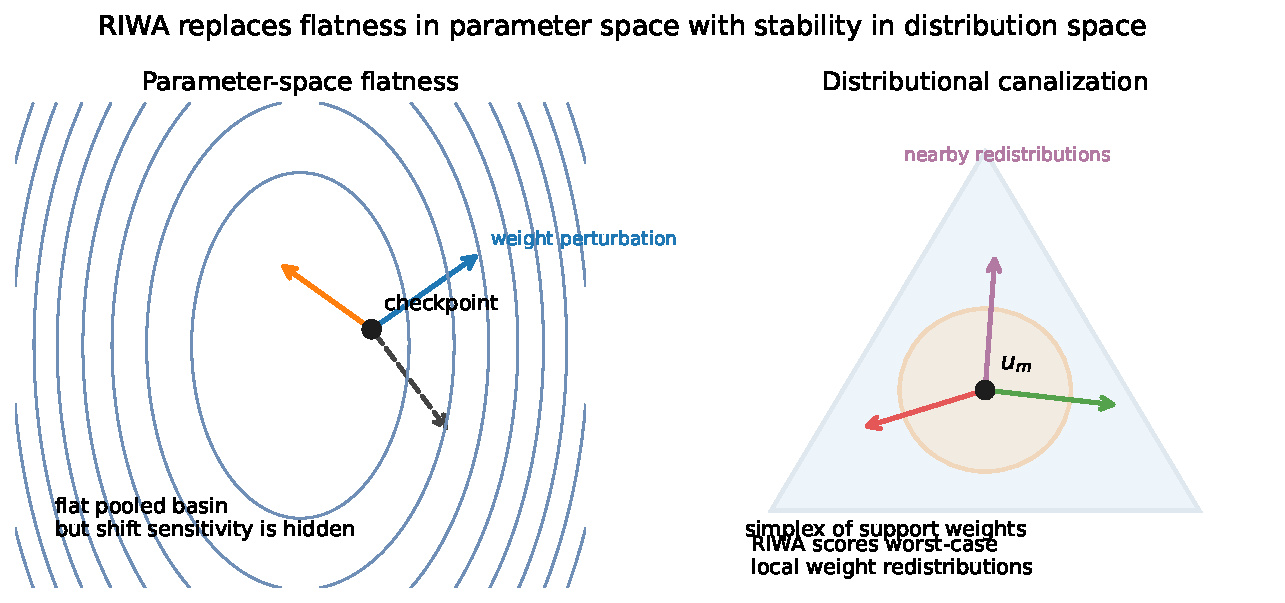
\includegraphics[width=\linewidth]{figures/distributional_canalization_vs_flatness.pdf}
    \caption{\textbf{Conceptual shift from flatness to canalization.} \swad{} probes stability to parameter perturbations around a pooled objective. \riwa{} instead probes stability to nearby \emph{support redistributions}: unseen domains are modeled locally as reweightings in the simplex of source support.}
    \label{fig:concept}
\end{figure}

\section{Related Work}

\paragraph{Single-run post-hoc DG.}
\swad{} \citep{cha2021wad} is the canonical single-run post-hoc DG method. Its impact comes from a compelling recipe: dense checkpoints, overfit-aware windowing, and final weight averaging. DiWA \citep{rame2022diwa} shows that more diverse model averages can outperform \swad{}, but the strongest results rely on combining many independently trained models or runs. \riwa{} stays in the same operational regime as \swad{} and changes the selector, not the training budget.

\paragraph{Weight averaging and flatness.}
SWA \citep{izmailov2018swa} and mode-connectivity work \citep{garipov2018fge} established that averaging along a trajectory often finds wider optima with good generalization. \swad{} imports this logic into DG. Our goal is not to discard that line, but to show that DG offers another natural invariance target: local shift directions in data-distribution space.

\paragraph{Influence, data reweighting, and local DRO.}
Influence functions quantify how losses change when individual training examples are infinitesimally reweighted \citep{koh2017influence}. DRO studies worst-case risk over ambiguity sets around a nominal distribution, often defined by $\chi^2$ or related divergences \citep{duchi2020variance,duchi2021learning}. \riwa{} draws from both: it defines a post-hoc robust one-step score over a local reweighting ball and evaluates checkpoints by their worst-case validation sensitivity.

\paragraph{Invariant directions and stability.}
Tangent Prop explicitly regularized derivatives along nuisance transformations \citep{simard1991tangent}. Algorithmic stability theory, while developed in a different language, also links low sensitivity to perturbations with generalization \citep{bousquet2002stability}. \riwa{} may be read as a post-hoc stability criterion, but the perturbations are not weight perturbations or individual deletions; they are nearby redistributions of source support mass.

\paragraph{Training-time transfer objectives.}
Meta-learning inspired DG methods such as MLDG \citep{li2018mldg} already exploit the principle that one source split should help another after a tiny update. Our earlier \rowa{} proposal used that idea directly but required domain labels. \riwa{} keeps the one-step-transfer spirit while removing the need for explicit domains: the latent shift is modeled at the level of sample weights instead of domain IDs.

\section{Reweighting-Invariant Weight Averaging}
\label{sec:method}

Assume a single training trajectory with checkpoints $\{\theta_t\}_{t=1}^{K}$. For model selection, we reserve two fixed held-out sets:
\begin{itemize}[leftmargin=1.4em]
    \item a support set $U = \{z_i\}_{i=1}^{m}$ used to emulate local source-mixture perturbations, and
    \item a validation set $V = \{v_j\}_{j=1}^{n}$ used to score the perturbed checkpoint.
\end{itemize}
No domain labels are required.

At checkpoint $\theta_t$, define
\begin{align}
    g_{i,t} &\triangleq \nabla_\theta \ell(z_i;\theta_t),\\
    \bar g_t &\triangleq \frac{1}{m}\sum_{i=1}^{m} g_{i,t},\\
    L_{V,t}(\theta) &\triangleq \frac{1}{n}\sum_{j=1}^{n} \ell(v_j;\theta),\\
    g_{V,t} &\triangleq \nabla_\theta L_{V,t}(\theta_t).
\end{align}
Let $P_t \succeq 0$ be an optional positive semidefinite preconditioner. The simplest choice is $P_t = I$; a diagonal second-moment or empirical-Fisher approximation is a practical alternative.

\subsection{Local ambiguity set in sample-weight space}

Let $u_m \triangleq \frac{1}{m}\mathbf{1} \in \RR^m$ denote uniform weights. For a radius $\rho \in (0,1/m]$, define the local ambiguity set
\begin{equation}
    \mathcal{A}_{\rho}
    \triangleq
    \left\{
    \alpha \in \simplex^m :
    \norm{\alpha - u_m}_2 \le \rho
    \right\}.
\end{equation}
The weighted support gradient is
\begin{equation}
    g_{U,t}(\alpha)
    \triangleq
    \sum_{i=1}^{m}\alpha_i g_{i,t}
    =
    \bar g_t + \sum_{i=1}^{m}(\alpha_i - 1/m)(g_{i,t}-\bar g_t).
\end{equation}
The virtual update induced by $\alpha$ is
\begin{equation}
    \theta_t(\alpha) \triangleq \theta_t - \eta P_t g_{U,t}(\alpha),
\end{equation}
where $\eta > 0$ is a small step size.

\subsection{Exact robust score}

The exact \riwa{} score is the worst-case validation loss after the virtual update:
\begin{equation}
    S_t^{\mathrm{ex}}(\eta,\rho)
    \triangleq
    \max_{\alpha \in \mathcal{A}_{\rho}}
    L_{V,t}(\theta_t(\alpha)).
    \label{eq:exact_score}
\end{equation}
This is the checkpoint-selection objective. Intuitively, a checkpoint is good when no nearby redistribution of support mass can make a tiny source-family step look bad on validation.

\subsection{First-order closed-form score}

Define the centered perturbation coefficients
\begin{equation}
    a_{i,t} \triangleq \inner{g_{V,t}}{P_t(g_{i,t}-\bar g_t)},
    \qquad
    a_t \triangleq (a_{1,t},\dots,a_{m,t})^\top.
\end{equation}
The first-order robust surrogate is
\begin{equation}
    S_t^{\mathrm{fo}}(\eta,\rho)
    \triangleq
    \max_{\alpha \in \mathcal{A}_{\rho}}
    \left[
    L_{V,t}(\theta_t) - \eta \inner{g_{V,t}}{P_t g_{U,t}(\alpha)}
    \right].
\end{equation}
In Section~\ref{sec:theory}, we show that this optimization has the exact closed form
\begin{equation}
    S_t^{\mathrm{fo}}(\eta,\rho)
    =
    L_{V,t}(\theta_t)
    -
    \eta \inner{g_{V,t}}{P_t \bar g_t}
    +
    \eta \rho \norm{a_t}_2.
    \label{eq:fo_score}
\end{equation}
If
\begin{equation}
    C_t
    \triangleq
    \frac{1}{m}\sum_{i=1}^{m}(g_{i,t}-\bar g_t)(g_{i,t}-\bar g_t)^\top
\end{equation}
is the support-gradient covariance, then Eq.~\eqref{eq:fo_score} is equivalently
\begin{equation}
    S_t^{\mathrm{fo}}(\eta,\rho)
    =
    L_{V,t}(\theta_t)
    -
    \eta \inner{g_{V,t}}{P_t \bar g_t}
    +
    \eta \rho \sqrt{m\, g_{V,t}^\top P_t C_t P_t g_{V,t}}.
    \label{eq:fo_covariance}
\end{equation}
The second term rewards validation-aligned descent; the third penalizes sensitivity to latent support shifts.

\subsection{Checkpoint selection and averaging}

Let $S_t$ denote either $S_t^{\mathrm{ex}}$ or $S_t^{\mathrm{fo}}$. We select
\begin{equation}
    t^\star \in \argmin_{1 \le t \le K} S_t
\end{equation}
and form a contiguous low-score window
\begin{equation}
    W_{\delta}
    \triangleq
    \left\{
    t : S_t \le S_{t^\star} + \delta
    \right\},
\end{equation}
restricted to the connected component containing $t^\star$. The final model is the average
\begin{equation}
    \bar \theta_{\riwa}
    \triangleq
    \sum_{t \in W_{\delta}} w_t \theta_t,
    \qquad
    w_t \ge 0,\quad \sum_{t \in W_{\delta}} w_t = 1.
\end{equation}
Uniform weights are the default.

\begin{figure*}[t]
    \centering
    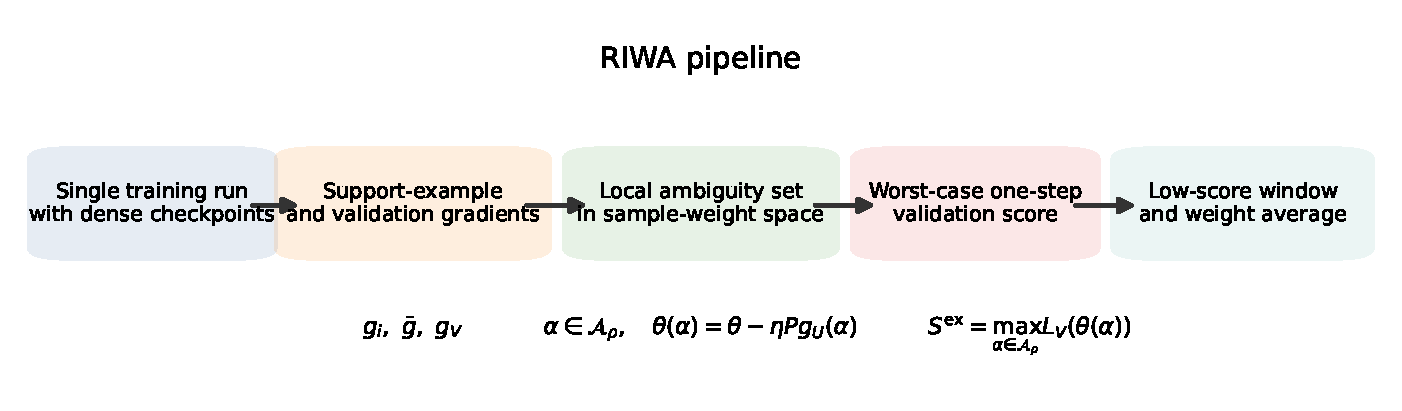
\includegraphics[width=0.96\textwidth]{figures/riwa_pipeline.pdf}
    \caption{\textbf{\riwa{} pipeline.} A single ordinary training run produces dense checkpoints. For each checkpoint, \riwa{} computes support-example gradients, forms a local ambiguity set over sample weights, scores the checkpoint by the worst-case validation loss after a tiny virtual update, and averages a contiguous low-score window.}
    \label{fig:pipeline}
\end{figure*}

\begin{algorithm}[t]
    \caption{\riwa{} (\textsc{Reweighting-Invariant Weight Averaging})}
    \label{alg:riwa}
    \begin{algorithmic}[1]
        \Require Checkpoints $\{\theta_t\}_{t=1}^{K}$ from one training run; held-out support set $U$; held-out validation set $V$; step size $\eta$; radius $\rho$; window width $\delta$; preconditioners $\{P_t\}_{t=1}^{K}$
        \For{$t=1,\dots,K$}
            \State Compute $g_{i,t} = \nabla_\theta \ell(z_i;\theta_t)$ for all $z_i \in U$
            \State $\bar g_t \gets \frac{1}{m}\sum_i g_{i,t}$
            \State Compute $L_{V,t}(\theta_t)$ and $g_{V,t} = \nabla_\theta L_{V,t}(\theta_t)$
            \If{exact score}
                \State $S_t \gets \max_{\alpha \in \mathcal{A}_{\rho}} L_{V,t}\!\left(\theta_t - \eta P_t g_{U,t}(\alpha)\right)$
            \Else
                \State $a_{i,t} \gets \inner{g_{V,t}}{P_t(g_{i,t}-\bar g_t)}$ for all $i$
                \State $S_t \gets L_{V,t}(\theta_t) - \eta\inner{g_{V,t}}{P_t \bar g_t} + \eta \rho \norm{a_t}_2$
            \EndIf
        \EndFor
        \State $t^\star \gets \argmin_t S_t$
        \State $W_{\delta} \gets$ connected sublevel window around $t^\star$
        \State \Return $\bar \theta_{\riwa} = \sum_{t \in W_{\delta}} w_t \theta_t$
    \end{algorithmic}
\end{algorithm}

\paragraph{Practical complexity.}
The exact score requires per-example support gradients and repeated evaluations of validation loss under virtual updates. The first-order score only needs support-example gradients, the mean support gradient, and one validation gradient. Since the score depends on the projected covariance direction $g_{V,t}^\top P_t(\cdot)$, practical implementations can use exact per-example gradients, micro-batch approximations, or last-layer-only gradients without changing the algorithmic form.

\section{Theory}
\label{sec:theory}

We now analyze \riwa{} under explicit local assumptions. The key point is that the method is not a heuristic penalty on top of flatness; it is a local robust objective over distribution perturbations.

\subsection{The ambiguity set is a local chi-square ball}

\begin{proposition}[Equivalence between centered $\ell_2$ and local $\chi^2$ ambiguity sets]
\label{prop:chisq}
Let $u_m = \frac{1}{m}\mathbf{1}$ and let $\alpha \in \simplex^m$. Then
\begin{equation}
    D_{\chi^2}(\alpha \,\|\, u_m)
    \triangleq
    \sum_{i=1}^{m}\frac{(\alpha_i - 1/m)^2}{1/m}
    =
    m \norm{\alpha - u_m}_2^2.
\end{equation}
Consequently,
\begin{equation}
    \mathcal{A}_{\rho}
    =
    \left\{
    \alpha \in \simplex^m :
    D_{\chi^2}(\alpha \,\|\, u_m) \le m\rho^2
    \right\}.
\end{equation}
\end{proposition}

Proposition~\ref{prop:chisq} is the first bridge to DRO: \riwa{} evaluates robustness to a local $\chi^2$ neighborhood around the empirical source support.

\subsection{Exact first-order robust score}

\begin{theorem}[Closed form of the first-order \riwa{} score]
\label{thm:support}
Fix a checkpoint $\theta_t$ and assume $\rho \le 1/m$. Then
\begin{equation}
    S_t^{\mathrm{fo}}(\eta,\rho)
    =
    L_{V,t}(\theta_t)
    -
    \eta \inner{g_{V,t}}{P_t \bar g_t}
    +
    \eta \rho \norm{a_t}_2,
\end{equation}
where $a_{i,t} = \inner{g_{V,t}}{P_t(g_{i,t}-\bar g_t)}$. Equivalently,
\begin{equation}
    S_t^{\mathrm{fo}}(\eta,\rho)
    =
    L_{V,t}(\theta_t)
    -
    \eta \inner{g_{V,t}}{P_t \bar g_t}
    +
    \eta \rho \sqrt{m\, g_{V,t}^\top P_t C_t P_t g_{V,t}}.
\end{equation}
\end{theorem}

Theorem~\ref{thm:support} shows that the first-order score is the support function of the centered ambiguity set. This is the precise sense in which \riwa{} seeks \emph{distributional tangent invariance}: it penalizes directional derivatives of the post-update validation loss along local reweighting directions.

\subsection{Exact-score upper bound}

\begin{assumption}[Validation smoothness]
\label{ass:smooth}
For every checkpoint under consideration, the validation loss $L_{V,t}$ is $\beta$-smooth in a neighborhood of $\theta_t$:
\begin{equation}
    L_{V,t}(\theta + \Delta)
    \le
    L_{V,t}(\theta)
    +
    \inner{\nabla L_{V,t}(\theta)}{\Delta}
    +
    \frac{\beta}{2}\norm{\Delta}_2^2
    \qquad
    \text{for all relevant } \theta,\Delta.
\end{equation}
\end{assumption}

\begin{theorem}[Smoothness upper bound for the exact \riwa{} score]
\label{thm:smooth}
Under Assumption~\ref{ass:smooth}, define
\begin{equation}
    \kappa_t(P_t)
    \triangleq
    \sqrt{m\, \lambda_{\max}(P_t C_t P_t)}.
\end{equation}
Then
\begin{equation}
    S_t^{\mathrm{ex}}(\eta,\rho)
    \le
    S_t^{\mathrm{fo}}(\eta,\rho)
    +
    \frac{\beta \eta^2}{2}
    \left(
        \norm{P_t \bar g_t}_2 + \rho \kappa_t(P_t)
    \right)^2.
    \label{eq:smooth_upper}
\end{equation}
\end{theorem}

Theorem~\ref{thm:smooth} is the main finite-step guarantee: the closed-form first-order score is not a loose intuition but a valid upper envelope of the exact robust objective up to a local quadratic remainder.

\begin{corollary}[Sufficient condition for robust improvement]
\label{cor:improve}
Under Assumption~\ref{ass:smooth}, if
\begin{equation}
    \inner{g_{V,t}}{P_t \bar g_t}
    >
    \rho \sqrt{m\, g_{V,t}^\top P_t C_t P_t g_{V,t}}
    +
    \frac{\beta \eta}{2}
    \left(
        \norm{P_t \bar g_t}_2 + \rho \kappa_t(P_t)
    \right)^2,
\end{equation}
then
\begin{equation}
    S_t^{\mathrm{ex}}(\eta,\rho)
    <
    L_{V,t}(\theta_t).
\end{equation}
\end{corollary}

Corollary~\ref{cor:improve} gives the interpretation most relevant to practice: a tiny support-family update remains beneficial under all nearby redistributions when mean descent dominates distributional sensitivity plus curvature.

\begin{figure}[t]
    \centering
    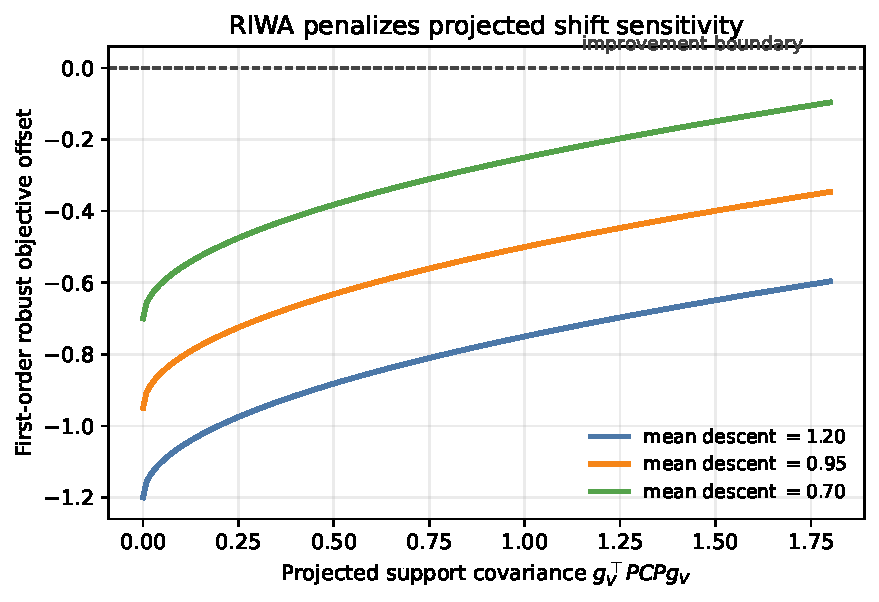
\includegraphics[width=\linewidth]{figures/projected_covariance_tradeoff.pdf}
    \caption{\textbf{The robust-improvement trade-off in Theorem~\ref{thm:smooth}.} \riwa{} prefers checkpoints with large validation-aligned mean descent and small projected support covariance. The same pooled loss can hide very different sensitivity profiles.}
    \label{fig:tradeoff}
\end{figure}

\subsection{Population target and plug-in consistency}

To interpret \riwa{} as a population object, define a support distribution $P_U$, a validation distribution $P_V$, the population support gradient mean
\begin{equation}
    \mu(\theta) \triangleq \EE_{z \sim P_U}[\nabla \ell(z;\theta)],
\end{equation}
the support-gradient covariance
\begin{equation}
    \Sigma(\theta)
    \triangleq
    \EE_{z \sim P_U}\left[
    (\nabla \ell(z;\theta)-\mu(\theta))(\nabla \ell(z;\theta)-\mu(\theta))^\top
    \right],
\end{equation}
and the validation gradient
\begin{equation}
    \nu(\theta) \triangleq \nabla L_V(\theta), \qquad L_V(\theta) \triangleq \EE_{v \sim P_V}[\ell(v;\theta)].
\end{equation}
For a fixed shift budget $\varepsilon > 0$, define the population first-order robust score
\begin{equation}
    \mathcal{S}_{\varepsilon}^{\mathrm{pop}}(\theta)
    \triangleq
    L_V(\theta)
    -
    \eta \nu(\theta)^\top P \mu(\theta)
    +
    \eta \sqrt{\varepsilon\, \nu(\theta)^\top P \Sigma(\theta) P \nu(\theta)}.
    \label{eq:population_score}
\end{equation}

\begin{proposition}[Plug-in consistency of the empirical first-order score]
\label{prop:consistency}
Fix $\theta$ and $P \succeq 0$. Let $U_m = \{z_i\}_{i=1}^{m}$ and $V_n = \{v_j\}_{j=1}^{n}$ be independent \iid{} samples from $P_U$ and $P_V$. Assume $\EE \norm{\nabla \ell(z;\theta)}_2^2 < \infty$ and $\EE \ell(v;\theta)^2 < \infty$. Define
\begin{align}
    \hat L_{V,n}(\theta) &\triangleq \frac{1}{n}\sum_{j=1}^{n}\ell(v_j;\theta),\\
    \hat \mu_m(\theta) &\triangleq \frac{1}{m}\sum_{i=1}^{m}\nabla \ell(z_i;\theta),\\
    \hat \nu_n(\theta) &\triangleq \nabla \hat L_{V,n}(\theta),\\
    \hat \Sigma_m(\theta) &\triangleq \frac{1}{m}\sum_{i=1}^{m}\left(\nabla \ell(z_i;\theta)-\hat \mu_m(\theta)\right)\left(\nabla \ell(z_i;\theta)-\hat \mu_m(\theta)\right)^\top.
\end{align}
Then the empirical score
\begin{equation}
    \hat{\mathcal{S}}_{m,n}^{\mathrm{fo}}(\theta)
    \triangleq
    \hat L_{V,n}(\theta)
    -
    \eta \hat \nu_n(\theta)^\top P \hat \mu_m(\theta)
    +
    \eta \sqrt{\varepsilon\, \hat \nu_n(\theta)^\top P \hat \Sigma_m(\theta) P \hat \nu_n(\theta)}
\end{equation}
converges almost surely to $\mathcal{S}_{\varepsilon}^{\mathrm{pop}}(\theta)$ as $m,n \to \infty$.
\end{proposition}

Proposition~\ref{prop:consistency} shows that \riwa{} is not merely finite-sample bookkeeping. With the natural scaling $\rho_m = \sqrt{\varepsilon/m}$, the empirical first-order score is a consistent estimator of a population robust objective.

\subsection{Why pooled flatness is not enough}

The next theorem is the key comparison result.

\begin{theorem}[Constructive separation from pooled-flatness selectors]
\label{thm:separation}
Fix $m=2$, $P=I$, $\rho \in (0,1/2]$, and nonzero $r \in \RR^p$. Let the validation loss be
\begin{equation}
    L_V(\theta + \Delta)
    =
    \ell_V + r^\top \Delta + \frac{\gamma}{2}\norm{\Delta}_2^2
\end{equation}
for some $\gamma > 0$. Consider two support families:
\begin{align}
    \ell_1^{A}(\theta+\Delta) &= c + r^\top \Delta + \frac{\beta}{2}\norm{\Delta}_2^2,\\
    \ell_2^{A}(\theta+\Delta) &= c + r^\top \Delta + \frac{\beta}{2}\norm{\Delta}_2^2,
\end{align}
and
\begin{align}
    \ell_1^{B}(\theta+\Delta) &= c + (1+\xi) r^\top \Delta + \frac{\beta}{2}\norm{\Delta}_2^2,\\
    \ell_2^{B}(\theta+\Delta) &= c + (1-\xi) r^\top \Delta + \frac{\beta}{2}\norm{\Delta}_2^2,
\end{align}
where $\xi > 0$.
Then:
\begin{enumerate}[label=(\roman*), leftmargin=1.5em]
    \item The pooled support loss is identical in the two families:
    \begin{equation}
        \frac{1}{2}\left(\ell_1^A + \ell_2^A\right)(\theta+\Delta)
        =
        \frac{1}{2}\left(\ell_1^B + \ell_2^B\right)(\theta+\Delta)
        =
        c + r^\top \Delta + \frac{\beta}{2}\norm{\Delta}_2^2.
    \end{equation}
    Hence the two families have the same pooled empirical loss, pooled gradient, and pooled Hessian at every local point.
    \item Their first-order \riwa{} scores differ strictly:
    \begin{equation}
        S_{B}^{\mathrm{fo}}(\eta,\rho)
        =
        S_{A}^{\mathrm{fo}}(\eta,\rho)
        +
        \eta \rho \sqrt{2}\,\xi \norm{r}_2^2.
        \label{eq:first_gap}
    \end{equation}
    \item If
    \begin{equation}
        0 < \eta < \frac{1}{\gamma(1+\sqrt{2}\xi\rho)},
        \label{eq:eta_condition}
    \end{equation}
    then their exact robust scores also satisfy
    \begin{equation}
        S_{B}^{\mathrm{ex}}(\eta,\rho)
        =
        S_{A}^{\mathrm{ex}}(\eta,\rho)
        +
        \sqrt{2}\xi\rho \eta \norm{r}_2^2(1-\gamma\eta)
        +
        \gamma \xi^2 \rho^2 \eta^2 \norm{r}_2^2
        >
        S_{A}^{\mathrm{ex}}(\eta,\rho).
        \label{eq:exact_gap}
    \end{equation}
\end{enumerate}
\end{theorem}

Theorem~\ref{thm:separation} shows exactly where \riwa{} is more informative than \swad{}-style pooled-flatness selection. The two checkpoints look identical from the viewpoint of pooled loss geometry, but one is much more vulnerable to local source redistributions. \riwa{} detects this vulnerability; any selector that only sees pooled flatness does not.

\subsection{Dense checkpointing and averaging}

\begin{proposition}[Dense checkpoint selection converges to the continuous optimum]
\label{prop:dense}
Let $\theta:[0,T] \to \RR^p$ be a continuous training trajectory and let $s(t) \triangleq S(\theta(t))$ be an $L_s$-Lipschitz score along the trajectory. Suppose checkpoints are saved at times $0=t_1<\cdots<t_K=T$ with maximum gap $\Delta = \max_k (t_{k+1}-t_k)$. Then
\begin{equation}
    \min_{1 \le k \le K}s(t_k)
    \le
    \min_{t \in [0,T]}s(t) + \frac{L_s \Delta}{2}.
\end{equation}
\end{proposition}

\begin{proposition}[Window averaging is safe under a local convex upper model]
\label{prop:avg}
Suppose a selected window $\{\theta_t\}_{t \in W}$ lies in a convex neighborhood on which an upper model of the exact \riwa{} score has the quadratic form
\begin{equation}
    U(\theta) = c + b^\top \theta + \frac{1}{2}\theta^\top Q \theta,
    \qquad Q \succeq 0.
\end{equation}
Then for any convex weights $\{w_t\}_{t \in W}$,
\begin{equation}
    U\!\left(\sum_{t \in W} w_t \theta_t\right)
    \le
    \sum_{t \in W} w_t U(\theta_t).
\end{equation}
\end{proposition}

Propositions~\ref{prop:dense} and \ref{prop:avg} justify the same practical scaffold that made \swad{} attractive: dense checkpointing plus averaging inside one low-score connected region.

\begin{figure}[t]
    \centering
    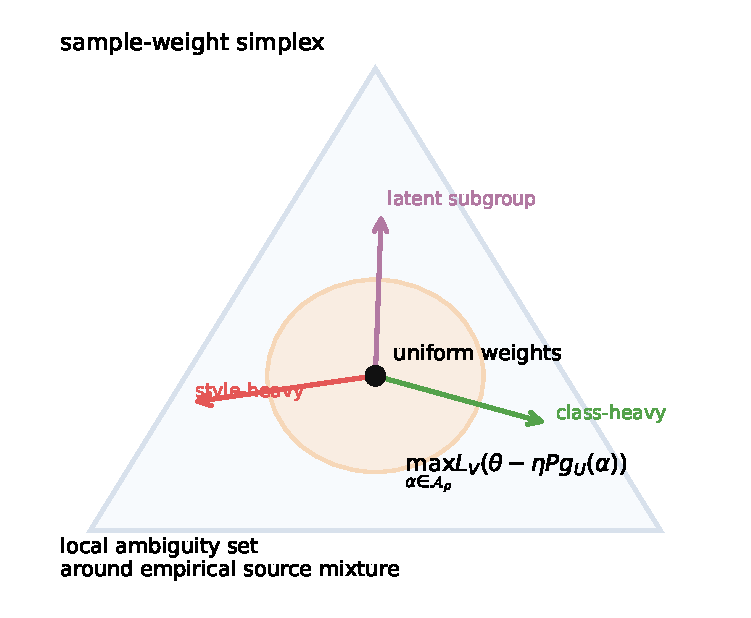
\includegraphics[width=\linewidth]{figures/weight_simplex_ambiguity.pdf}
    \caption{\textbf{The ambiguity set for \riwa{}.} The method scores each checkpoint by the worst-case direction in a small neighborhood of uniform support weights. The local adversary operates in the simplex of sample weights, not in parameter space.}
    \label{fig:simplex}
\end{figure}

\section{Experimental Protocol}
\label{sec:experiments}

This paper is complete as a method and theory manuscript, but the new \riwa{} experiments have not yet been run. The quantitative sections below are therefore intentionally structured as a protocol plus published reference targets.

\subsection{Benchmarks and backbone}

We will evaluate on the five standard DomainBed datasets used by \swad{} and DiWA: PACS \citep{li2017pacs}, VLCS \citep{fang2013vlcs}, OfficeHome \citep{venkateswara2017officehome}, TerraIncognita \citep{beery2018terraincognita}, and DomainNet \citep{peng2019domainnet}. Following prior work \citep{cha2021wad,rame2022diwa,gulrajani2021in}, the primary backbone is ResNet-50 and the primary protocol is leave-one-domain-out evaluation with model selection on held-out source validation data.

\subsection{Baselines}

We will compare against:
\begin{itemize}[leftmargin=1.4em]
    \item ERM, the DomainBed reference baseline \citep{gulrajani2021in};
    \item CORAL \citep{sun2016coral};
    \item SWA \citep{izmailov2018swa};
    \item \swad{} \citep{cha2021wad};
    \item DiWA \citep{rame2022diwa};
    \item optional auxiliary comparisons against SAM \citep{foret2021};
    \item our earlier domain-labeled post-hoc baseline \rowa{} for ablation only, not as the primary comparison.
\end{itemize}

\subsection{\riwa{} variants}

The main planned variants are:
\begin{itemize}[leftmargin=1.4em]
    \item \textbf{\riwa-FO}: first-order score, identity preconditioner;
    \item \textbf{\riwa-FO-Diag}: first-order score, diagonal preconditioner;
    \item \textbf{\riwa-Exact}: exact score with inner maximization over $\mathcal{A}_{\rho}$;
    \item \textbf{\riwa-Single}: best single checkpoint without averaging;
    \item \textbf{\riwa-Window}: the default contiguous low-score average.
\end{itemize}

The primary hyperparameters are the virtual step size $\eta$, the ambiguity radius $\rho$ (or the equivalent $\chi^2$ budget $\varepsilon = m\rho^2$), and the sublevel width $\delta$.

\subsection{Metrics}

We will report:
\begin{itemize}[leftmargin=1.4em]
    \item mean \ood{} accuracy;
    \item mean \iid{} validation accuracy on held-out source validation data;
    \item worst-domain \ood{} accuracy;
    \item Spearman correlation between checkpoint score and final \ood{} accuracy;
    \item added compute relative to \swad{}.
\end{itemize}

\subsection{Falsifiable predictions}

The theory makes clear, falsifiable predictions:
\begin{enumerate}[leftmargin=1.4em]
    \item \riwa{} score should correlate with \ood{} accuracy more strongly than pooled-flatness proxies when projected support covariance is substantial.
    \item \riwa-FO should recover most of the gain of \riwa-Exact when selected checkpoints lie in a smooth local regime.
    \item Window averaging should outperform single-checkpoint selection whenever the best checkpoints form one connected low-score region.
    \item Gains over \swad{} should be largest on benchmarks where latent support shift dominates pure parameter-space flatness effects.
\end{enumerate}

\begin{figure}[t]
    \centering
    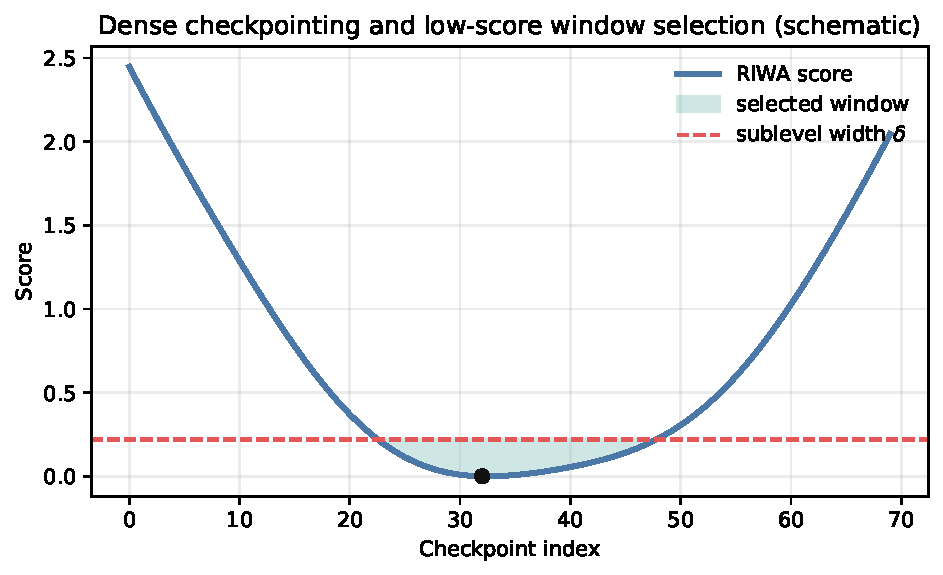
\includegraphics[width=\linewidth]{figures/dense_window_schematic.pdf}
    \caption{\textbf{Dense checkpoint sampling and low-score window averaging.} \riwa{} preserves the same practical recipe that made \swad{} easy to adopt: dense checkpointing and averaging inside one contiguous low-score region. The figure is schematic, not empirical.}
    \label{fig:window}
\end{figure}

\section{Published Reference Results and Placeholder Tables}
\label{sec:results}

We include exact published baselines from prior work so that the empirical target is clear before running \riwa{}. Every new \riwa{} row is intentionally marked as \TBD{}.

\begin{table*}[t]
    \centering
    \small
    \setlength{\tabcolsep}{5pt}
    \caption{\textbf{Published reference results on DomainBed with ResNet-50.} Numbers are copied from the cited papers and are included here as reference targets for the planned \riwa{} evaluation.}
    \label{tab:published}
    \begin{tabular}{lcccccc}
        \toprule
        Method & PACS & VLCS & OfficeHome & TerraInc & DomainNet & Avg \\
        \midrule
        ERM \citep{cha2021wad,rame2022diwa} & 85.5 & 77.5 & 66.5 & 46.1 & 40.9 & 63.3 \\
        CORAL \citep{rame2022diwa} & 86.2 & 78.8 & 68.7 & 47.6 & 41.5 & 64.6 \\
        \swad{} \citep{cha2021wad} & 88.1 & 79.1 & 70.6 & 50.0 & 46.5 & 66.9 \\
        CORAL + \swad{} \citep{cha2021wad} & 88.3 & 78.9 & 71.3 & 51.0 & 46.8 & 67.3 \\
        DiWA (random init, $M=60$) \citep{rame2022diwa} & 89.0 & 79.4 & 71.6 & 49.0 & 46.3 & 67.1 \\
        DiWA (LP init, $M=60$) \citep{rame2022diwa} & 89.0 & 78.6 & 72.8 & 51.9 & 47.7 & 68.0 \\
        \midrule
        \riwa-FO (ours) & \TBD & \TBD & \TBD & \TBD & \TBD & \TBD \\
        \riwa-FO-Diag (ours) & \TBD & \TBD & \TBD & \TBD & \TBD & \TBD \\
        \riwa-Exact (ours) & \TBD & \TBD & \TBD & \TBD & \TBD & \TBD \\
        \bottomrule
    \end{tabular}
\end{table*}

\begin{table}[t]
    \centering
    \small
    \setlength{\tabcolsep}{3.0pt}
    \renewcommand{\arraystretch}{1.15}
    \caption{\textbf{Published \swad{} ablation results copied from \citet{cha2021wad}.} These numbers motivate the dense-window design that \riwa{} inherits.}
    \label{tab:swad_ablation}
    \adjustbox{max width=\linewidth}{
    \begin{tabular}{@{}l|cccc|ccc|ccc@{}}
        \toprule
        & \multicolumn{4}{c|}{Configuration} & \multicolumn{3}{c|}{Out-of-domain} & \multicolumn{3}{c}{In-domain} \\
        & $t_s$ & $t_e$ & lr & interval & PACS & VLCS & Avg. & PACS & VLCS & Avg. \\
        \midrule
        SWA$_{\text{w/ cyclic}}$ & 4000 & 5000 & Cyclic & 100 & 85.9 $\pm 0.1$ & 76.6 $\pm 0.1$ & 81.2 & 97.1 $\pm 0.1$ & 85.0 $\pm 0.2$ & 91.0 \\
        SWA$_{\text{w/ const}}$ & 4000 & 5000 & Const & 100 & 86.5 $\pm 0.3$ & 76.7 $\pm 0.2$ & 81.6 & 97.3 $\pm 0.1$ & 85.0 $\pm 0.2$ & 91.1 \\
        SWAD$_{\text{w/o Dense}}$ & Opt & Overfit & Const & 100 & 86.5 $\pm 0.4$ & 78.0 $\pm 0.7$ & 82.2 & 97.6 $\pm 0.1$ & 85.8 $\pm 0.4$ & 91.7 \\
        SWAD$_{\text{w/o Opt-Overfit}}$ & 4000 & 5000 & Const & 1 & 86.6 $\pm 0.6$ & 76.9 $\pm 0.3$ & 81.7 & 97.5 $\pm 0.1$ & 85.2 $\pm 0.1$ & 91.3 \\
        SWAD$_{\text{w/o Overfit}}$ & Opt & 5000 & Const & 1 & 87.1 $\pm 0.3$ & 77.6 $\pm 0.1$ & 82.4 & 97.7 $\pm 0.1$ & 85.8 $\pm 0.3$ & 91.8 \\
        SWAD$_{\text{fit-on-val}}$ & Val & Val & Const & 1 & 86.2 $\pm 0.2$ & 78.6 $\pm 0.1$ & 82.4 & 97.5 $\pm 0.2$ & 85.8 $\pm 0.3$ & 91.7 \\
        SWAD (proposed) & Opt & Overfit & Const & 1 & 87.1 $\pm 0.2$ & 78.9 $\pm 0.2$ & 83.0 & 97.7 $\pm 0.1$ & 86.1 $\pm 0.5$ & 91.9 \\
        \bottomrule
    \end{tabular}
    }
\end{table}

\begin{table*}[t]
    \centering
    \small
    \caption{\textbf{Planned main results table.} Every \riwa{} cell remains intentionally left as \TBD{} until experiments are run.}
    \label{tab:main_tbd}
    \begin{tabular}{lcccccc}
        \toprule
        Method & PACS & VLCS & OfficeHome & TerraInc & DomainNet & Avg \\
        \midrule
        \swad{} & 88.1 & 79.1 & 70.6 & 50.0 & 46.5 & 66.9 \\
        DiWA (best published) & 89.0 & 78.6 & 72.8 & 51.9 & 47.7 & 68.0 \\
        \riwa-FO & \TBD & \TBD & \TBD & \TBD & \TBD & \TBD \\
        \riwa-FO-Diag & \TBD & \TBD & \TBD & \TBD & \TBD & \TBD \\
        \riwa-Exact & \TBD & \TBD & \TBD & \TBD & \TBD & \TBD \\
        \bottomrule
    \end{tabular}
\end{table*}

\begin{table}[t]
    \centering
    \small
    \caption{\textbf{Planned \riwa{} ablations.} These rows are intentionally blank pending experiments.}
    \label{tab:ablations}
    \begin{tabular}{lc}
        \toprule
        Ablation & Avg \\
        \midrule
        \riwa-FO vs. \riwa-Exact & \TBD \\
        Identity vs. diagonal preconditioner & \TBD \\
        Single checkpoint vs. low-score window & \TBD \\
        Support subset size sensitivity & \TBD \\
        Score/\ood{} correlation & \TBD \\
        Compute overhead vs. \swad{} & \TBD \\
        \bottomrule
    \end{tabular}
\end{table}

\paragraph{What the theory predicts.}
Before any experiment is run, the theory already implies a sharp empirical question: do the checkpoints that minimize local reweighting sensitivity outperform those that only minimize pooled-flatness surrogates? If the answer is yes, the gain should be largest when projected support covariance is substantial and not largest when it is already negligible.

\section{Discussion and Limitations}

\paragraph{Why \riwa{} could outperform \swad{}.}
\swad{} seeks flatness in parameter space. \riwa{} seeks invariance to local source-mixture perturbations in distribution space. If unseen domains are well approximated by small redistributions of latent support components, then \riwa{} is better aligned with the actual DG target because its score is an explicit local robust objective over those perturbations. Theorems~\ref{thm:support} and \ref{thm:separation} make this precise.

\paragraph{Why \riwa{} may fail.}
The same clarity also exposes its limits. If the test shift lies far outside the local support hull, a local reweighting criterion may be too weak. If per-example gradients are too noisy, the projected covariance term may be poorly estimated. If label shift dominates covariate or style redistribution, the local simplex perturbation model may mis-specify the shift.

\paragraph{What the theory proves.}
The theory proves four concrete facts. First, \riwa{} is exactly a local $\chi^2$-DRO selector at first order. Second, its exact robust score is upper-bounded by a closed-form smoothness envelope. Third, its empirical first-order score is a consistent plug-in estimator of a population robust objective. Fourth, pooled-flatness selectors can be blind to local distributional sensitivity that \riwa{} captures.

\paragraph{What the theory does not prove.}
The theory does not prove universal empirical superiority over \swad{}, DiWA, or any other DG method. It cannot. Any such claim without experiments would be irresponsible. The value of the theory is that it identifies a concrete failure mode of flatness-only selection and supplies a simple post-hoc selector that directly targets that failure mode.

\paragraph{Current practical limitation.}
The obvious current limitation is empirical: the experiments have not yet been executed. The manuscript is therefore publication-style and method-complete, but it is not submission-complete as an empirical claim until the \TBD{} results are replaced by real numbers.

\section{Conclusion}

We proposed \riwa{}, a label-free single-run post-hoc DG method based on distributional canalization rather than pooled flatness. The method scores checkpoints by worst-case validation behavior under local support reweightings, then averages a contiguous low-score window. Our theory shows that \riwa{} is a local robust objective in distribution space, admits an exact first-order closed form, has a controlled exact-score upper bound, is statistically well defined, and detects sensitivity patterns that flatness-only selectors cannot. The empirical section remains to be executed, but the manuscript now contains the method, the theory, the figures, the protocol, and the published reference baselines needed to do so.

\bibliographystyle{unsrtnat}
\bibliography{references}

\appendix

\section{Detailed Proofs}

\subsection{Proof of Proposition~\ref{prop:chisq}}

\begin{proof}
By definition of the $\chi^2$ divergence with reference distribution $u_m$,
\begin{equation}
    D_{\chi^2}(\alpha \,\|\, u_m)
    =
    \sum_{i=1}^{m}\frac{(\alpha_i - 1/m)^2}{1/m}
    =
    m\sum_{i=1}^{m}(\alpha_i - 1/m)^2
    =
    m\norm{\alpha - u_m}_2^2.
\end{equation}
Therefore
\begin{equation}
    \norm{\alpha - u_m}_2 \le \rho
    \iff
    D_{\chi^2}(\alpha \,\|\, u_m) \le m\rho^2.
\end{equation}
Intersecting with $\simplex^m$ yields the claim.
\end{proof}

\subsection{Proof of Theorem~\ref{thm:support}}

\begin{proof}
Because $\rho \le 1/m$, every vector $\delta \in \RR^m$ satisfying $\mathbf{1}^\top \delta = 0$ and $\norm{\delta}_2 \le \rho$ gives $\alpha = u_m + \delta \in \simplex^m$, since each coordinate obeys
\begin{equation}
    \alpha_i = \frac{1}{m} + \delta_i \ge \frac{1}{m} - \norm{\delta}_\infty \ge \frac{1}{m} - \rho \ge 0.
\end{equation}
Therefore $\mathcal{A}_{\rho}$ may be parameterized as
\begin{equation}
    \mathcal{A}_{\rho}
    =
    \left\{
    u_m + \delta :
    \mathbf{1}^\top \delta = 0,\ \norm{\delta}_2 \le \rho
    \right\}.
\end{equation}
For such an $\alpha$,
\begin{align}
    \inner{g_{V,t}}{P_t g_{U,t}(\alpha)}
    &=
    \inner{g_{V,t}}{P_t \bar g_t}
    +
    \sum_{i=1}^{m}\delta_i \inner{g_{V,t}}{P_t(g_{i,t}-\bar g_t)} \\
    &=
    \inner{g_{V,t}}{P_t \bar g_t} + \delta^\top a_t.
\end{align}
Hence
\begin{align}
    S_t^{\mathrm{fo}}(\eta,\rho)
    &=
    \max_{\mathbf{1}^\top \delta = 0,\ \norm{\delta}_2 \le \rho}
    \left[
    L_{V,t}(\theta_t)
    -
    \eta \inner{g_{V,t}}{P_t \bar g_t}
    -
    \eta \delta^\top a_t
    \right].
\end{align}
The vector $a_t$ is centered because
\begin{equation}
    \mathbf{1}^\top a_t
    =
    \sum_{i=1}^{m}\inner{g_{V,t}}{P_t(g_{i,t}-\bar g_t)}
    =
    \inner{g_{V,t}}{P_t\sum_{i=1}^{m}(g_{i,t}-\bar g_t)}
    = 0.
\end{equation}
Therefore the constraint $\mathbf{1}^\top \delta = 0$ does not reduce the support function, and Cauchy--Schwarz yields
\begin{equation}
    \max_{\mathbf{1}^\top \delta = 0,\ \norm{\delta}_2 \le \rho} (-\delta^\top a_t)
    =
    \rho \norm{a_t}_2,
\end{equation}
attained at $\delta^\star = -\rho a_t / \norm{a_t}_2$ when $a_t \neq 0$.
This proves
\begin{equation}
    S_t^{\mathrm{fo}}(\eta,\rho)
    =
    L_{V,t}(\theta_t)
    -
    \eta \inner{g_{V,t}}{P_t \bar g_t}
    +
    \eta \rho \norm{a_t}_2.
\end{equation}

For the covariance form,
\begin{align}
    \norm{a_t}_2^2
    &=
    \sum_{i=1}^{m}
    \inner{g_{V,t}}{P_t(g_{i,t}-\bar g_t)}^2 \\
    &=
    g_{V,t}^\top P_t
    \left(
    \sum_{i=1}^{m}(g_{i,t}-\bar g_t)(g_{i,t}-\bar g_t)^\top
    \right)
    P_t g_{V,t} \\
    &=
    m\, g_{V,t}^\top P_t C_t P_t g_{V,t}.
\end{align}
Substituting into the first expression proves the equivalent covariance form.
\end{proof}

\subsection{Proof of Theorem~\ref{thm:smooth}}

\begin{proof}
Fix $\alpha \in \mathcal{A}_{\rho}$ and let $\Delta(\alpha) = -\eta P_t g_{U,t}(\alpha)$. By Assumption~\ref{ass:smooth},
\begin{equation}
    L_{V,t}(\theta_t + \Delta(\alpha))
    \le
    L_{V,t}(\theta_t)
    +
    \inner{g_{V,t}}{\Delta(\alpha)}
    +
    \frac{\beta}{2}\norm{\Delta(\alpha)}_2^2.
\end{equation}
Since $\Delta(\alpha) = -\eta P_t g_{U,t}(\alpha)$,
\begin{equation}
    L_{V,t}(\theta_t(\alpha))
    \le
    L_{V,t}(\theta_t)
    -
    \eta \inner{g_{V,t}}{P_t g_{U,t}(\alpha)}
    +
    \frac{\beta \eta^2}{2}\norm{P_t g_{U,t}(\alpha)}_2^2.
\end{equation}
Taking the maximum over $\alpha \in \mathcal{A}_{\rho}$ gives
\begin{equation}
    S_t^{\mathrm{ex}}(\eta,\rho)
    \le
    S_t^{\mathrm{fo}}(\eta,\rho)
    +
    \frac{\beta \eta^2}{2}
    \max_{\alpha \in \mathcal{A}_{\rho}}\norm{P_t g_{U,t}(\alpha)}_2^2.
\end{equation}
Write $\alpha = u_m + \delta$. Then
\begin{equation}
    g_{U,t}(\alpha)
    =
    \bar g_t + G_t \delta,
\end{equation}
where $G_t \in \RR^{p \times m}$ has columns $g_{i,t}-\bar g_t$. Hence
\begin{align}
    \norm{P_t g_{U,t}(\alpha)}_2
    &\le
    \norm{P_t \bar g_t}_2 + \norm{P_t G_t \delta}_2 \\
    &\le
    \norm{P_t \bar g_t}_2 + \norm{P_t G_t}_{\mathrm{op}}\norm{\delta}_2 \\
    &\le
    \norm{P_t \bar g_t}_2 + \rho \norm{P_t G_t}_{\mathrm{op}}.
\end{align}
It remains to identify $\norm{P_t G_t}_{\mathrm{op}}$. Because $P_t$ is symmetric,
\begin{align}
    \norm{P_t G_t}_{\mathrm{op}}^2
    &=
    \lambda_{\max}(G_t^\top P_t^2 G_t).
\end{align}
The nonzero eigenvalues of $G_t^\top P_t^2 G_t$ equal those of $P_t G_t G_t^\top P_t$. Since $G_t G_t^\top = m C_t$, we obtain
\begin{equation}
    \norm{P_t G_t}_{\mathrm{op}}^2
    =
    m\, \lambda_{\max}(P_t C_t P_t)
    =
    \kappa_t(P_t)^2.
\end{equation}
Therefore
\begin{equation}
    \max_{\alpha \in \mathcal{A}_{\rho}}\norm{P_t g_{U,t}(\alpha)}_2
    \le
    \norm{P_t \bar g_t}_2 + \rho \kappa_t(P_t),
\end{equation}
and substituting this into the previous inequality proves Eq.~\eqref{eq:smooth_upper}.
\end{proof}

\subsection{Proof of Corollary~\ref{cor:improve}}

\begin{proof}
By Theorem~\ref{thm:smooth},
\begin{align}
    S_t^{\mathrm{ex}}(\eta,\rho)
    &\le
    L_{V,t}(\theta_t)
    -
    \eta \inner{g_{V,t}}{P_t \bar g_t}
    +
    \eta \rho \sqrt{m\, g_{V,t}^\top P_t C_t P_t g_{V,t}} \nonumber\\
    &\qquad +
    \frac{\beta \eta^2}{2}
    \left(
        \norm{P_t \bar g_t}_2 + \rho \kappa_t(P_t)
    \right)^2.
\end{align}
The stated inequality makes the right-hand side strictly less than $L_{V,t}(\theta_t)$, which proves the claim.
\end{proof}

\subsection{Proof of Proposition~\ref{prop:consistency}}

\begin{proof}
By the strong law of large numbers,
\begin{align}
    \hat L_{V,n}(\theta) &\to L_V(\theta) \quad \text{a.s.},\\
    \hat \mu_m(\theta) &\to \mu(\theta) \quad \text{a.s.},\\
    \hat \nu_n(\theta) &\to \nu(\theta) \quad \text{a.s.}
\end{align}
as $m,n \to \infty$. Likewise, each entry of the empirical second-moment matrix
\begin{equation}
    \frac{1}{m}\sum_{i=1}^{m}\nabla \ell(z_i;\theta)\nabla \ell(z_i;\theta)^\top
    \to
    \EE\left[\nabla \ell(z;\theta)\nabla \ell(z;\theta)^\top\right]
    \quad \text{a.s.}
\end{equation}
Since
\begin{equation}
    \hat \Sigma_m(\theta)
    =
    \frac{1}{m}\sum_{i=1}^{m}\nabla \ell(z_i;\theta)\nabla \ell(z_i;\theta)^\top
    -
    \hat \mu_m(\theta)\hat \mu_m(\theta)^\top,
\end{equation}
we obtain
\begin{equation}
    \hat \Sigma_m(\theta) \to \Sigma(\theta) \quad \text{a.s.}
\end{equation}
Matrix multiplication and the square-root map are continuous on the cone of positive semidefinite matrices, so
\begin{equation}
    \hat \nu_n(\theta)^\top P \hat \Sigma_m(\theta) P \hat \nu_n(\theta)
    \to
    \nu(\theta)^\top P \Sigma(\theta) P \nu(\theta)
    \quad \text{a.s.}
\end{equation}
Finally, the map
\begin{equation}
    (x,y,z,w) \mapsto x - \eta y^\top P z + \eta \sqrt{\varepsilon\, y^\top P w P y}
\end{equation}
is continuous on the relevant domain, so the continuous mapping theorem yields
\begin{equation}
    \hat{\mathcal{S}}_{m,n}^{\mathrm{fo}}(\theta)
    \to
    \mathcal{S}_{\varepsilon}^{\mathrm{pop}}(\theta)
    \quad \text{a.s.}
\end{equation}
\end{proof}

\subsection{Proof of Theorem~\ref{thm:separation}}

\begin{proof}
We prove the three parts in order.

\paragraph{Part (i).}
For family $A$,
\begin{equation}
    \frac{1}{2}\left(\ell_1^A + \ell_2^A\right)(\theta+\Delta)
    =
    c + r^\top \Delta + \frac{\beta}{2}\norm{\Delta}_2^2.
\end{equation}
For family $B$,
\begin{align}
    \frac{1}{2}\left(\ell_1^B + \ell_2^B\right)(\theta+\Delta)
    &=
    \frac{1}{2}
    \left[
        c + (1+\xi)r^\top \Delta + \frac{\beta}{2}\norm{\Delta}_2^2
        +
        c + (1-\xi)r^\top \Delta + \frac{\beta}{2}\norm{\Delta}_2^2
    \right] \\
    &=
    c + r^\top \Delta + \frac{\beta}{2}\norm{\Delta}_2^2.
\end{align}
Thus the pooled support loss, gradient, and Hessian are identical.

\paragraph{Part (ii).}
At $\Delta = 0$, family $A$ has support gradients
\begin{equation}
    g_1^A = g_2^A = r,
    \qquad
    \bar g^A = r.
\end{equation}
Therefore $a^A = 0$ and
\begin{equation}
    S_A^{\mathrm{fo}}(\eta,\rho)
    =
    \ell_V - \eta \norm{r}_2^2.
\end{equation}
Family $B$ has
\begin{equation}
    g_1^B = (1+\xi)r,
    \qquad
    g_2^B = (1-\xi)r,
    \qquad
    \bar g^B = r.
\end{equation}
Hence
\begin{equation}
    a_1^B = \inner{r}{(g_1^B-\bar g^B)} = \xi \norm{r}_2^2,
    \qquad
    a_2^B = -\xi \norm{r}_2^2.
\end{equation}
So
\begin{equation}
    \norm{a^B}_2 = \sqrt{2}\,\xi \norm{r}_2^2.
\end{equation}
Applying Theorem~\ref{thm:support},
\begin{equation}
    S_B^{\mathrm{fo}}(\eta,\rho)
    =
    \ell_V - \eta \norm{r}_2^2 + \eta \rho \sqrt{2}\,\xi \norm{r}_2^2,
\end{equation}
which proves Eq.~\eqref{eq:first_gap}.

\paragraph{Part (iii).}
Any $\alpha \in \mathcal{A}_{\rho}$ can be written as
\begin{equation}
    \alpha = \left(\frac{1}{2}+s,\ \frac{1}{2}-s\right),
    \qquad
    |s| \le \frac{\rho}{\sqrt{2}}.
\end{equation}
For family $A$, the weighted support gradient is always $r$, so
\begin{equation}
    S_A^{\mathrm{ex}}(\eta,\rho)
    =
    L_V(\theta - \eta r)
    =
    \ell_V - \eta \norm{r}_2^2 + \frac{\gamma \eta^2}{2}\norm{r}_2^2.
\end{equation}
For family $B$, the weighted support gradient becomes
\begin{align}
    g_U^B(\alpha)
    &=
    \left(\frac{1}{2}+s\right)(1+\xi)r + \left(\frac{1}{2}-s\right)(1-\xi)r \\
    &=
    (1+2\xi s)r.
\end{align}
Hence
\begin{equation}
    L_V(\theta - \eta g_U^B(\alpha))
    =
    \ell_V - \eta (1+2\xi s)\norm{r}_2^2 + \frac{\gamma \eta^2}{2}(1+2\xi s)^2 \norm{r}_2^2.
\end{equation}
Differentiate with respect to $s$:
\begin{equation}
    \frac{d}{ds}
    L_V(\theta - \eta g_U^B(\alpha))
    =
    2\xi \eta \norm{r}_2^2
    \left(
        -1 + \gamma \eta (1+2\xi s)
    \right).
\end{equation}
If Eq.~\eqref{eq:eta_condition} holds, then for all feasible $s$,
\begin{equation}
    \gamma \eta (1+2\xi s)
    \le
    \gamma \eta (1+\sqrt{2}\xi \rho)
    < 1,
\end{equation}
so the derivative is strictly negative. Therefore the maximum occurs at the smallest feasible $s$, namely $s^\star = -\rho/\sqrt{2}$. Substituting this value gives
\begin{equation}
    S_B^{\mathrm{ex}}(\eta,\rho)
    =
    \ell_V - \eta (1-\sqrt{2}\xi\rho)\norm{r}_2^2 + \frac{\gamma \eta^2}{2}(1-\sqrt{2}\xi\rho)^2 \norm{r}_2^2.
\end{equation}
Subtracting $S_A^{\mathrm{ex}}(\eta,\rho)$ yields
\begin{align}
    S_B^{\mathrm{ex}}(\eta,\rho) - S_A^{\mathrm{ex}}(\eta,\rho)
    &=
    \sqrt{2}\xi\rho \eta \norm{r}_2^2
    +
    \frac{\gamma \eta^2}{2}
    \left[
        (1-\sqrt{2}\xi\rho)^2 - 1
    \right]
    \norm{r}_2^2 \\
    &=
    \sqrt{2}\xi\rho \eta \norm{r}_2^2(1-\gamma\eta)
    +
    \gamma \xi^2 \rho^2 \eta^2 \norm{r}_2^2.
\end{align}
The right-hand side is strictly positive because Eq.~\eqref{eq:eta_condition} implies $\eta < 1/\gamma$.
\end{proof}

\subsection{Proof of Proposition~\ref{prop:dense}}

\begin{proof}
Let $t^\star \in \argmin_{t \in [0,T]} s(t)$. Choose a checkpoint $t_k$ such that $|t_k - t^\star| \le \Delta/2$, which exists by construction of the grid. By Lipschitz continuity,
\begin{equation}
    s(t_k)
    \le
    s(t^\star) + L_s |t_k - t^\star|
    \le
    s(t^\star) + \frac{L_s \Delta}{2}.
\end{equation}
Taking the minimum over $k$ proves the claim.
\end{proof}

\subsection{Proof of Proposition~\ref{prop:avg}}

\begin{proof}
Since $Q \succeq 0$, the function
\begin{equation}
    U(\theta) = c + b^\top \theta + \frac{1}{2}\theta^\top Q \theta
\end{equation}
is convex. Jensen's inequality therefore gives
\begin{equation}
    U\!\left(\sum_{t \in W} w_t \theta_t\right)
    \le
    \sum_{t \in W} w_t U(\theta_t)
\end{equation}
for any nonnegative weights summing to one.
\end{proof}

\section{Additional Notes for Implementation}

\paragraph{Exact inner maximization.}
The exact score in Eq.~\eqref{eq:exact_score} is a low-dimensional smooth maximization problem over the simplex neighborhood $\mathcal{A}_{\rho}$. In practice, projected gradient ascent over the weight vector $\alpha$ is sufficient because the inner problem dimension is the size of the support subset, not the parameter dimension.

\paragraph{Diagonal preconditioning.}
The default theory uses a symmetric positive semidefinite $P_t$. A practical diagonal choice is
\begin{equation}
    P_t = \diag(\hat v_t + \tau)^{-1/2},
\end{equation}
where $\hat v_t$ is the optimizer second-moment state or a diagonal empirical Fisher and $\tau > 0$ is a damping term.

\paragraph{Why the method is label-free.}
Neither the score nor the theory uses source-domain identifiers. The ambiguity set is defined over support-example weights, so the method can be applied wherever one has differentiable losses and held-out support/validation splits.

\paragraph{What must be implemented carefully.}
The main numerical sensitivity is the projected covariance term
\begin{equation}
    g_{V,t}^\top P_t C_t P_t g_{V,t}.
\end{equation}
If per-example gradients are very noisy, support subsampling or averaged micro-batches should be used to stabilize its estimation.

\end{document}
